\documentclass[a4paper,11pt]{article}
\usepackage{cmap}
\usepackage{polski}
\usepackage[T1]{fontenc}
\usepackage[utf8]{inputenc}
\usepackage{graphicx}
\usepackage{minted}
\usepackage{titlesec}

\titlelabel{\thetitle.\quad}

\date{
{Data zajęć: 26.11.2017\hfill Data oddania: 24.01.2018}
\\
{Termin zajęć: Pon. TP 9:15\hfill Prowadzący zajęcia: Mgr inż. Szymon Datko}
}
\title{Sprawozdanie nr 4}
\author{Jakub Majewski 238902}

\makeatletter
\renewcommand{\maketitle}{
   \begin{titlepage}
     \begin{center}
       {\@date}
       \\
       \par\vspace{3ex}
       {\LARGE\@title}
       \par\vspace{1ex}
       \begin{tabular}[t]{c}
         \@author
       \end{tabular}
     \end{center}
     \@thanks
   \end{titlepage}
}
\makeatother

\begin{document}

\begin{center}\Large
    Grafika Komputerowa i Komunikacja Człowiek-Komputer
\end{center}

\hrule
    {\let\newpage\relax\maketitle}
\hrule

\section{Opis tematu}

Temat: OpenGL - Oświetlenie scen 3-D. \\ \\
Zrealizowane zadania: \\
1. stworzenie pojedynczego źródła światła przy użyciu biblioteki OpenGL, \\
2. stworzenie tablicy wektorów normalnych dla własnego modelu, \\
3. dodanie drugiego źródła światła o innej barwie. \\

\newpage
\section{Opis najważniejszych fragmentów kodu}

1. Metody klasy 'Light' odpowiedzialnej za tworzenie pojedynczego źródła światła.

\begin{minted}[linenos,tabsize=2,breaklines]{CPP}
Light::Light(int idx ) : idx(idx), glIdx(glIdx),
	light_position{ 0.0, 0.0, 10.0, 1.0 }, 
	light_ambient{ 0.0, 0.0, 0.0, 1.0 },
	light_diffuse{ 1.0, 1.0, 1.0, 1.0 }, 
	light_specular{ 1.0, 1.0, 1.0, 1.0 },
	att_constant{ 0.f }, att_linear{ 0.f }, 
	att_quadratic{ 0.f } {;}

// Inicjalizacja światła z domyślnymi parametrami
void Light::Init() {
	glLightfv(glIdx, GL_AMBIENT, light_ambient);
	glLightfv(glIdx, GL_DIFFUSE, light_diffuse);
	glLightfv(glIdx, GL_SPECULAR, light_specular);
	glLightfv(glIdx, GL_POSITION, light_position);
	glLightf(glIdx, GL_CONSTANT_ATTENUATION, att_constant);
	glLightf(glIdx, GL_LINEAR_ATTENUATION, att_linear);
	glLightf(glIdx, GL_QUADRATIC_ATTENUATION, att_quadratic);
}

Light& Light::SetCLQ(float c, float l, float q) {
	att_constant = c; att_linear = l; att_quadratic = q;
	glLightf(glIdx, GL_CONSTANT_ATTENUATION, att_constant);
	glLightf(glIdx, GL_LINEAR_ATTENUATION, att_linear);
	glLightf(glIdx, GL_QUADRATIC_ATTENUATION, att_quadratic);
	return *this;
}

Light& Light::SetPosition(float x, float y, float z) {
	light_position[0] = x;
	light_position[1] = y;
	light_position[2] = z;
	glLightfv(glIdx, GL_POSITION, light_position);
	return *this;
}

// Analogicznie jak dla SetAmbient:
Light& Light::SetAmbient(float x, float y, float z) {...}
Light& Light::SetDiffuse(float x, float y, float z) {...}
Light& Light::SetSpecular(float x, float y, float z) {...}

\end{minted}
\newpage

\noindent 2. Klasa 'LightManager' odpowiedzialna za przechowywanie i tworzenie \\
nowych źródeł światła. Umożliwia również modyfikowanie parametrów już stworzonych świateł.

\begin{minted}[linenos,tabsize=2,breaklines]{CPP}
struct LightManager {

	GLfloat mat_ambient[4];
	GLfloat mat_diffuse[4];
	GLfloat mat_specular[4];
	GLfloat mat_shininess;

	std::vector<std::unique_ptr<Light>> lights;

	LightManager() :		
		mat_ambient{ 0.2, 0.2, 0.2, 1.0 },
		mat_diffuse{ 1.0, 1.0, 1.0, 1.0 },
		mat_specular{ 1.0, 1.0, 1.0, 1.0 },
		mat_shininess{ 100.0 } {;}

    // Inicjalizacja silnika świateł OpenGL oraz parametrów powierzchni
	void Init() {

		glMaterialfv(GL_FRONT, GL_SPECULAR, mat_specular);
		glMaterialfv(GL_FRONT, GL_AMBIENT, mat_ambient);
		glMaterialfv(GL_FRONT, GL_DIFFUSE, mat_diffuse);
		glMaterialf(GL_FRONT, GL_SHININESS, mat_shininess);
		glShadeModel(GL_SMOOTH);
		glEnable(GL_LIGHTING);
		glEnable(GL_DEPTH_TEST);
	}

    // Zwracanie istniejącego już światła
	Light* GetLight(int idx) {
		return lights[idx].get();
	}

    // Tworzenie nowego światła
	Light* CreateLight() {
		glEnable(GL_LIGHT0+lights.size());
		lights.emplace_back(new Light(lights.size()))->Init();
		return lights.back().get();
	}
};
\end{minted}

\newpage

\noindent 2. Metody w odpowiedzialne za wygenerowanie przestrzeni wektorów normalnych renderowanego obiektu.

\begin{minted}[linenos,tabsize=2,breaklines]{CPP}
void Egg::calculateTU(float *tu, float u, float v) {
	tu[0] = (-450.f * u*u*u*u + 900.f * u*u*u - 810.f * u*u + 360.f * u - 45.f) * std::cos(3.14159f*v);
	tu[1] = (640.f * u*u*u - 960.f * u*u + 320.f * u);
	tu[2] = (-450.f * u*u*u*u + 900.f * u*u*u - 810.f * u*u + 360.f * u - 45.f) * std::sin(3.14159f*v);
}

void Egg::calculateTV(float *tv, float u, float v) {
	tv[0] = 3.14159*(90.f * u*u*u*u*u - 225.f * u*u*u*u + 270.f * u*u*u - 180.f * u*u + 45.f * u) * std::sin(3.14159f*v);
	tv[1] = 0.f;
	tv[2] = -3.14159*(90.f * u*u*u*u*u - 225.f * u*u*u*u + 270.f * u*u*u - 180.f * u*u + 45.f * u) * std::cos(3.14159f*v);
}

void Egg::calculateNormalTab() {
	float tu[3]{}, tv[3]{};
	for (int i = 0; i < N; ++i) {
		for (int j = 0; j < N; ++j) {
			float u = float(i) / (N - 1);
			float v = float(j) / (N - 1);
			calculateTU(tu, u, v);
			calculateTV(tv, u, v);
			float *p = normalTab[i][j];
			p[0] = tu[1] * tv[2] - tu[2] * tv[1];
			p[1] = tu[2] * tv[0] - tu[0] * tv[2];
			p[2] = tu[0] * tv[1] - tu[1] * tv[0];
			float len = std::sqrt(p[0]*p[0]+p[1]*p[1]+ p[2]*p[2]);
	
			// Kod naprawiający, opisany we wnioskach
			if(i == 0 || i == N-1) p[1] = -1.f;
			else {		
				if (u >= 0.5f) len *= -1.f;				
				p[0] /= len;
				p[1] /= len;
				p[2] /= len;
			}
		}
	}
}
\end{minted}

\section{Rezultat pracy}

\begin{figure}[h!]
    \centering
    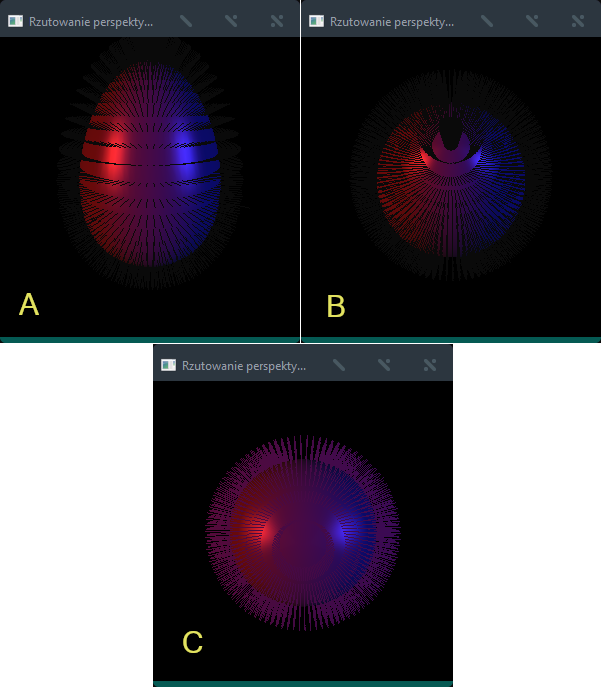
\includegraphics[width=1.0\linewidth]{screen.png}
    \caption{Obiekt oświetlony dwoma źródłami światła (o różnej barwie), obserwowany z boku (A), od góry (B) oraz od spodu (C)}
    \label{fig:screen1}
\end{figure}

\newpage

\section{Spostrzeżenia i wnioski}
Po stworzeniu przestrzeni wektorów normalnych promienie świetlne zaczęły się odbijać od obiektu w naturalny i prawidłowy sposób, ale na spodzie obiekt dalej nie był oświetlony. Wynikało to z faktu, że długość obliczonych wektorów normalnych na spodzie jajka była równa zero. W wyniku normalizowania wektorów (dzielenia ich parametrów przez długość wektora), parametry wektora osiągały wartości typu Nan. Problem rozwiązałem przez stworzenie w newralgicznych punktach sztucznych wektorów o parametrach [0, -1, 0].

\end{document}